% !TeX root = ../main.tex

\chapter{基于工具调用轨迹的知识图谱构建}

\section{引言}

本章介绍了一种基于工具调用轨迹数据进行工具知识图谱构造的策略,并基于此方法实现了一个大规模的工具知识图谱。本章将会围绕着工具知识图谱构建中的一些挑战出发,比如:
1.如何对工具调用轨迹数据进行数据筛选,得到高质量的工具集以及工具调用轨迹?
2.如何设计工具知识图谱的结构,以表示工具之间隐含的依赖关系?
3.如何验证工具图谱作为知识库的有效性?

基于上述问题,我们进行了以下研究:首先,我们提出了两种数据筛选策略,从API工具和API调用轨迹的角度对数据进行了筛选,保留了一批高质量的工具轨迹数据。
其次,我们设计了工具动态转移权值和工具静态转移权值两种方式,通过对工具轨迹数据进行计算,得到了工具之间的转换权值,用于后续指导大语言模型进行选择。
最后,关于验证工具图谱作为知识库的有效性,我们对比了直接用普通的检索增强方式和包含图谱知识的方式,验证了构建工具知识图谱的有效性。

\section{整体流程}

在现实场景的工具调用场景中,其实不同类型的工具之前存在隐含的顺序关系,比如“城市经纬度查询”和“根据经纬度获取实时天气”的工具总是在一起使用。这种存在于工具调用轨迹中的“过程性知识”对工具规划非常有启发性,能够表示工具之间的调用关系和跳转关系。基于此,我们希望能够通过对工具之间的转换关系进行建模,并将工具的搜索范围限定在一个更精确的空间,以辅助大语言模型工具调用。

我们分析了目前公开可用的通用工具学习数据集ToolBench、API-Bank,其中包含大量的多跳工具调用轨迹。通过分析其中的数据,我们发现每个工具后都只有一小部分后继工具会被调用,这证实了我们的观点,即工具之间存在相互调用的关系。

因此我们通过对开源的工具调用轨迹数据进行数据筛选、数据清洗等流程构建了一个大型的工具图谱。数据筛选和清洗流程中,本文制定了详细的规则,筛选得到高质量的工具推理轨迹作为图谱构建的基础数据。同时,我们设计了两种不同的图谱构建策略:静态和动态图谱构建,两种构建都对图谱上的转换权值进行修改,两种方法互相辅助表示工具之间的转换关系。在最终构建的图谱中,图上的节点为对应的开源工具,图上的边为有向边,标记了工具之间的跳转和调用关系,边上的权值为转换权值,即多有可能从当前工具跳转到下一工具。

在图谱建立后,我们将大量工具信息与工具之间的依赖关系表示与图谱上,并且通过在图谱上进行深度优先遍历或者广度优先遍历等方式选择合适的工具调用路径。关于图谱利用的部分会在下一章详细介绍。

\section{数据收集和清洗}

\subsection{数据集介绍}

目前较为大型的工具调用数据集有ToolBench\cite{Qin2023},API-Bank\cite{Li2023c},AgentBench\cite{Liu2023b}等。

AgentBench主要聚焦的是多情景的工具调用,比如。而本文侧重点在于真实世界的API工具,因此我们基于ToolBench和API-Bank构建了工具图谱。

ToolBench包括来自49个类别的16464个真实的RestAPI工具,并根据这些工具构建了包含126486条推理轨迹的数据集,共调用了469585个API。

ToolBench中使用的API都来自于一个开放的API托管平台“RapidAPI Hub”,在这个API托管平台中包含各种不同类别、不同供应商的API服务,需要订阅了相应的工具集才能够使用。在RapidAPI Hub中,工具以以下的方式进行组织,即网站上有不同的大类,大类下面会有不同的工具集,而工具集下面会有对应的单独的API工具。

【画图来展示rapidAPI hub的内容】

ToolBench中包含不同类型的数据,如:1.每个工具集的详细描述信息,包括工具集的名称、描述、类别等 2.工具的输入、输出参数列表 3.工具调用的示例代码 4.通过GPT-3.5生成的真实调用轨迹和参考API工具列表等等。

在本文中,为了构建工具知识图谱,因此我们在图谱构建部分主要利用的是通过GPT-3.5生成的工具调用轨迹数据。由于RapidAPI Hub上,同功能的工具可能有很多,即API工具之间存在着相似性或者能够从功能上相互替换,因此对于同一个用户任务,有多条路径都能够解决问题。因此对于每个需求,并不存在一个标准答案路径。但是我们可以通过分析最终的回答结果,判断经过一组API顺序调用之后系统输出的结果是否符合预期,来判断路径是否合理。

ToolBench的工具调用轨迹数据为一个树状遍历结构,如下所示。

【画图来展示轨迹数据结构】

\section{数据清洗}

通过大语言模型构建的工具调用轨迹数据可能会有重复调用/API工具编排错误等问题,
并且数据集中的工具调用是以决策树的方式组织的,需要从中获得正确的工具路径。
基于上述问题,我们对工具调用轨迹数据进行了一些清洗,主要筛选方式如下:

\begin{itemize}
  \item \textbf{删除失败工具调用轨迹}:工具调用轨迹数据最后会对用户需求进行正面解答或放弃,我们只保留成功调用的API工具调用轨迹,删除无法得到结果的工具调用轨迹。
  \item \textbf{删除过长工具调用轨迹}:通过数据分析,我们发现ToolBench中的工具轨迹数据的API路径长度不一,平均的调用路径长度为4,但是极个别的API工具调用路径长度达到了20。
  过长的工具调用轨迹通常表示提供给大语言模型智能体的工具无法很好地完成该任务,导致工具调用一直在失败,
  因此我们将工具调用轨迹数据长度作为筛选指标,筛选掉长度大于8的API调用轨迹。因为这些API调用轨迹的API工具数量过多,无法进行有效的图谱构建。
  \item \textbf{删除无效工具节点}:在筛选优质工具轨迹后,我们还需要对工具轨迹数据进行清洗,得到在决策树上的正确的那一条路径。主要分为两种方式:1.去重,即对于同一个工具,如果有多个API的重复调用,我们只保留最后一次该API的成功调用记录。2.删除失败工具,如果工具调用轨迹中存在工具调用失败的情况,那么我们从轨迹中删除该工具。最后得到的应该是一个线性的调用轨迹。
\end{itemize}

原始数据集中包含了xx条工具调用轨迹数据,
其中平均的工具调用次数为xxx次,
经过上述的筛选逻辑后,共剩下xxx条工具调用轨迹数据。
我们基于该高质量的轨迹数据集建立工具图谱。

\section{图谱构建}

工具图谱的构建对于系统整体的性能和效率至关重要。
在这里,我们参考了ToolNet当中的设计\cite{Liu2024}
将API工具作为图谱中的工具节点,
工具节点之间的边上带有一个权值,该权值叫做“工具转移权值”,用于代表
从当前工具出发,有多大的可能性会跳转到调用另一个工具的使用。
除了边上带有权值,工具节点自身也带有一个权值,该权值叫做“工具可用性权值”,用于表示该
工具的可用性。

因此,在该工具图谱中,权值的计算方式非常重要。边和点的权值应该有区分度,不然无法提供有效的信息。

我们首先将会介绍基于历史工具调用数据的静态图谱构建方式,由于API工具具有时效性和多变性,我们还会对图上的节点、节点权值还有边上的权值进行动态的更新。

\subsection{静态构建}

静态构建图的过程相对简单,只需要遍历轨迹数据,并计算每两个节点之间的边权和点权值即可。

设定 $D$ 为已完成任务的工具使用轨迹集合,每条轨迹由工具使用的顺序构成,

\[
\text{Trajectory} = [D_1, D_2, \ldots, D_n]
\]

假设每个工具的调用成功与否是一个二元变量 $x_i$,其中:

\[
x_i = 
\begin{cases} 
1, & \text{工具调用成功} \\
-1, & \text{工具调用失败}
\end{cases}
\]

为了简化操作,我们将“结束”视为一种普通工具,每个工具都与“结束”工具节点相连,
当大语言模型智能体认为要结束调用过程时,就会选择“结束”工具。

节点 $v_i$ 到 $v_j$ 的转移权重 $w_{i,j}$ 计算如下:

\[
w_{i,j} = \frac{\mathbb{E}_D[1(\text{tool}_s = v_i \land \text{tool}_{s+1} = v_j)]}{\mathbb{E}_D[1(\text{tool}_s = v_i)]}
\]

其中,$\mathbb{E}_D[\cdot]$ 表示对轨迹集合 $D$ 上的期望操作,$1(\cdot)$ 是指示函数,当条件满足时取值为1,否则为0。
该公式计算了工具 $v_i$ 被调用后紧接着调用工具 $v_j$ 的频率。

除了关注工具之间的依赖关系,每个单独的工具的可用性和稳定性也是真实场景下重要考虑因素。
在工具调用轨迹中,有一些工具调用会出现无访问权限或访问超时的错误信息。
因此我们在工具图中通过对节点的权值进行计算和定义,通过点权来表示该工具的可用性或稳定性。
节点 $v_i$ 的可用性权重 $\alpha_i$ 计算如下:

\[
\alpha_i = \frac{\sum_{s=1}^{n} 1(x_s = 1 \land \text{tool}_s = v_i)}{\sum_{s=1}^{n} 1(\text{tool}_s = v_i)} \quad (0 \leq \alpha_i \leq 1)
\]

这里,$\alpha_i$ 表示工具 $v_i$ 的调用成功率,是该工具在轨迹中成功调用的次数与其总调用次数的比值。
因此该权值的范围是0-1,越接近1,表示该工具的可用性越高,越接近0,表示该工具的可用性越低。

通过对筛选后的工具轨迹数据进行上述计算,我们得到了工具图谱的初始静态图谱。

\subsection{动态更新}

基于上述方法构建的静态工具图谱,本文还提出了对边权和点权的动态更新。
动态更新对于工具图谱的构建至关重要,原因主要包括以下几点:
1. \textbf{新工具的初始化与数据稀缺问题}:当一个新的 API 工具被引入时,由于缺乏历史调用数据,无法通过传统的静态方法来初始化它的节点信息。在许多场景下,工具使用轨迹的数据量往往十分有限。或者在加入了新的工具节点时,这些新加入的节点并没有工具调用轨迹数据,因此难以判断该工具与其他工具之间的跳转关系。因此,我们希望能够利用大语言模型(LLM)的内在知识来对这些新工具进行初步的节点初始化,解决数据稀缺问题,并为工具的进一步使用提供一个合理的起点。
2. \textbf{用户偏好的动态变化}:在实际应用中,随着用户行为的变化,新的调用轨迹会不断生成。这些新轨迹反映了用户的真实偏好,因此需要及时添加到工具图谱中,使其能够反映最新的用户需求。
3. \textbf{工具的生命周期变化}:工具是动态变化的,随着时间推移,有些工具可能会因为开发者的弃用或其他原因而逐渐失去支持。静态构建无法反映这些变化,而需要通过动态更新来调整图中的边权重,确保图谱能够保持对工具现状的准确性。

动态更新发生在两个时间节点:1.产生了新的工具调用轨迹 2.添加了新的工具到工具图谱。
以下是对于边权和点权更新的具体阐述。

\subsubsection{边权的动态更新}

动态更新过程

对图 \( G \) 的更新尤为关键。由于可用工具轨迹的数量有限,我们需要对每一条轨迹进行细致检查。
LLM 作为工具的评估者,将整个轨迹作为输入,评估每个工具节点的表现。

每个工具的评分范围为 \( [-3, 3] \) 的离散整数,
用于反映工具在调用过程中的表现。
我们用 \( \Delta_i^{(n)} \) 表示在第 \( n \) 次迭代中节点 \( v_i \) 的评估得分。
节点 \( v_i \) 的累积得分 \( s_i^{(n)} \) 计算如下:

\[
s_i^{(n)} = \sum_{k=1}^{n} \Delta_i^{(k)}
\]

该公式对节点 \( v_i \) 在每次迭代中的评分进行累积,为后续的转移权重更新提供基础。

转移权重的更新

节点 \( v_i \) 到 \( v_j \) 的转移权重 \( w_{i,j}^{(n)} \) 在第 \( n \) 次迭代中的更新公式如下:

\[
w_{i,j}^{(n)} = \beta w_{i,j}^{(0)} + (1 - \beta) \Delta w_{i,j}^{(n)}
\]

其中,\( w_{i,j}^{(0)} \) 是初始的转移权重,\( \beta \) 是控制初始权重与动态更新之间平衡的超参数,\( \Delta w_{i,j}^{(n)} \) 是用于更新转移权重的归一化梯度,计算公式如下:

\[
\Delta w_{i,j}^{(n)} = \frac{f(s_i^{(n)})}{\sum_{v_j \in \text{oneigh}(v_i)} f(s_j^{(n)})}
\]

该公式通过累积分数 \( s_i^{(n)} \) 和 \( s_j^{(n)} \) 来更新转移权重,确保工具之间的转移反映最新的评估结果。

\subsubsection{点权的动态更新}

在点权的动态更新中,我们通过分析新生成的工具调用轨迹来调整工具的可用性权重。设调用轨迹为:

\[
\text{Trajectory} = [D_1, D_2, \ldots, D_n]
\]

对于每个工具 \( D_i \) 的调用结果记作 \( x_i \),其中:

- \( x_i = -1 \) 表示调用出错,
- \( x_i = +1 \) 表示调用成功。

在这里,出错的调用情况指的是 API 工具本身存在可用性问题,例如遇到状态码“403 Forbidden”、“408 Request Timeout”等。

根据调用结果,我们可以对点权的分数进行更新。更新公式如下:

\[
v_i^{(n)} = \beta v_i^{(0)} + (1 - \beta) \Delta v_i^{(n)}
\]

其中:
- \( v_i^{(0)} \) 是工具 \( D_i \) 的初始权重,
- \( \beta \) 是控制初始权重与动态更新之间平衡的超参数,其值会根据错误信息的严重程度进行调整,
- \( \Delta v_i^{(n)} \) 是用于更新权重的归一化梯度,计算公式如下:

\[
\Delta v_i^{(n)} = \frac{f(s_i^{(n)})}{\sum_{D_j \in \text{oneigh}(D_i)} f(s_j^{(n)})}
\]

在此公式中,$f(s_i^{(n)})$ 是累积分数,通过反映工具 \( D_i \) 的评估结果,确保工具之间的转移权重反映最新的使用情况和反馈。

\subsubsection{分数映射函数}

函数 $f(x)$ 用于将累积分数映射到 $(0, +\infty)$ 的范围内,从而确保在权重更新过程中生成正值。归一化的必要性在于,它能够确保所有工具的表现有效比较,避免负值对权重更新造成不良影响。具体而言,映射函数确保所有工具的权重更新结果均为正值,这对于构建有效的工具图谱至关重要。同时,函数通过灵活处理正负分数,使算法在不同情境下保持良好表现,保持各工具之间的相对表现,从而提升模型的准确性和稳定性。函数定义如下:

\[
f(x) :=
\begin{cases}
\alpha x + 1, & \text{if } x \geq 0 \\
e^{\alpha x}, & \text{if } x < 0
\end{cases}
\]

在这个函数中,$\alpha$ 是控制映射函数行为的超参数。对于正分数,映射为线性函数 $f(x) = \alpha x + 1$,使得得分的正向提升以线性方式反映在权重更新中。对于负分数,映射为指数衰减函数 $f(x) = e^{\alpha x}$,这保证了即使在评分较低的情况下,权重的更新也会保持在一个合理的范围内。

\section{API召回模型训练}

通过对现有的通用向量模型进行测试,如BGE,BCE,M3E等,我们发现通用的向量模型在用户需求与工具匹配任务上具有一定提升空间。因此,本文提出了基于通用向量模型进行微调,提升模型在工具选择上的能力。

本文在训练数据构造部分提出了细粒度、高难度的正负样本构建策略,有效提升了模型的工具搜索能力。

\subsection{训练数据构造}

在训练向量模型时,训练数据包含三个部分:正样本,负样本,查询语句。
查询语句即为数据集中的“query”字段,对应用户输入的查询信息。
正样本也可以直接使用数据集提供的参考API列表。
但是对于负样本的部分,我们采取了两种不同的负样本构造方式:一种是简单负样本(Simple Negative)构造一种是困难负样本构造(Hard Negative)。

\indent \textbf{简单负样本构造}。对于简单负样本构造,我们直接选择了不同大类的K个工具作为负样本。

\indent \textbf{基于大语言模型的困难负样本构造}。在工具选择、调用场景,开源的通用向量模型难以区分工具之间细微的语义区别。

如下图所示,(介绍为什么需要tune,明明两个很不同的相似度很高,但是很一致的相似度很低)。

因此,困难负样本构造的目的是帮助模型更好地区分工具之间细微的语义区别,帮助更好地应对噪声。
我们选择采用GPT-3.5完成困难负样本的构造。由于原工具数据量众多,从中筛选语义表述类似、但是功能上有区别的工具样本费时费力。因此我们采取了直接用大语言模型生成工具描述作为负样本的策略。

具体策略如下:
首先,我们采样一批<query,推荐工具集>的数据,
然后我们遍历其中的推荐工具集的工具,
通过提示词将用户需求和工具描述提供给大语言模型,
要求模型生成类似但是功能上无法满足用户需求的工具描述。
通过这样遍历工具描述生成负样本,可以生成一组高质量的困难负样本供模型学习。

本文分别使用简单负样本构造和困难负样本构造方法构造了xxx条数据和xxx条数据,分别对模型进行了微调。
同时,在测试集中,我们除了使用从ToolBench中筛选得到的数据。

\subsection{模型训练及超参数设置}

在进行向量模型微调之前,选择合适的基座模型是一个关键步骤,这将直接影响到微调后模型的性能以及效率。在选择基座模型时,通常需要考虑到模型的规模、大小,模型支持的语言,模型的训练任务等。

基于上述原因,本工作在对比性能后选择了BGE-m3模型作为基础模型进行训练。理由如下:


本工作基于BGE-m3进行了微调。实现过程中将epoch数量设置为xx,学习率设置为3e-5进行学习。
模型大小为xxx,在xxx芯片上训练了xxx得到了结果。

\section{实验结果}



\begin{table}[!ht]
  \centering
  \caption{API工具召回实验结果}
  \label{tab:comparison}
  \begin{tabular}{lccc>{\bfseries}c} % 'lccc' defines 1 left and 3 center aligned columns, '>{\bfseries}c' makes last column bold
    \toprule
    \textbf{Method} & \textbf{I1} & \textbf{I2} & \textbf{I3} & \textbf{Average} \\ \midrule
    BCE         & 30.1 & 40.0 & 28.6 & 32.9 \\
    BGE-Small         & 42.3 & 45.6 & 33.2 & 40.4 \\
    ToolBench   & 46.5 & 49.1 & 38.9 & 44.8 \\
    Ours        & \textbf{58.0} & \textbf{70.6} & \textbf{62.8} & \textbf{63.8} \\ \bottomrule
  \end{tabular}
\end{table}

% \section{插图}

% 插图功能是利用 \TeX{} 的特定编译程序提供的机制实现的,不同的编译程序支持不同的图
% 形方式。有的同学可能听说“\LaTeX{} 只支持 EPS”,事实上这种说法是不准确的。\XeTeX{}
% 可以很方便地插入 EPS、PDF、PNG、JPEG 格式的图片。

% 一般图形都是处在浮动环境中。之所以称为浮动是指最终排版效果图形的位置不一定与源文
% 件中的位置对应,这也是刚使用 \LaTeX{} 同学可能遇到的问题。如果要强制固定浮动图形
% 的位置,请使用 \pkg{float} 宏包,它提供了 \texttt{[H]} 参数。

% \subsection{单个图形}

% 图要有图题,研究生图题采用中英文对照,并置于图的编号之后,图的编号和图题应置于图
% 下方的居中位置。引用图应在图题右上角标出文献来源。文中必须有关于本插图的提示,如
% “见图~\ref{fig:energy-distrib}”、“如图~\ref{fig:energy-distrib} 所示”等。该页空
% 白不够排写该图整体时,则可将其后文字部分提前排写,将图移到次页。

% \begin{figure}[!htp]
%   \centering
%   \begin{tikzpicture}
%     \begin{axis}[
%       width=12cm,
%       height=9cm,
%       xmin=0, xmax=7,
%       xlabel={$r$ (\unit{\milli\metre})},
%       ymin=-1000, ymax=11000,
%       ylabel={Energy (\unit[per-mode=symbol]{\watt\per\cubic\metre})},
%       scaled ticks=false,
%       tick label style={
%         /pgf/number format/1000 sep=,
%         font={\zihao{-5}},
%       },
%       minor tick num=1,
%       tick pos=left,
%       tick align=outside,
%       tick style={thin,black},
%     ]
%       \addplot [only marks,mark=square*] 
%         table [x={radial}, y={energy}, col sep=comma] 
%         {./assets/energy-distrib.csv};
%       \node at (2,6000) 
%         {$q_{v}=\dfrac{\sigma\omega^{2}|\mathbf{A}|^{2}}{2}$};
%     \end{axis}
%   \end{tikzpicture}
%   \bicaption{内热源沿径向的分布}{Energy distribution along radial}
%   \label{fig:energy-distrib}
% \end{figure}

% \subsection{多个图形}

% 简单插入多个图形的例子如图~\ref{fig:SRR} 所示。这两个水平并列放置的子图共用一个
% 图形计数器,没有各自的子图题。

% \begin{figure}[!htp]
%   \centering
%   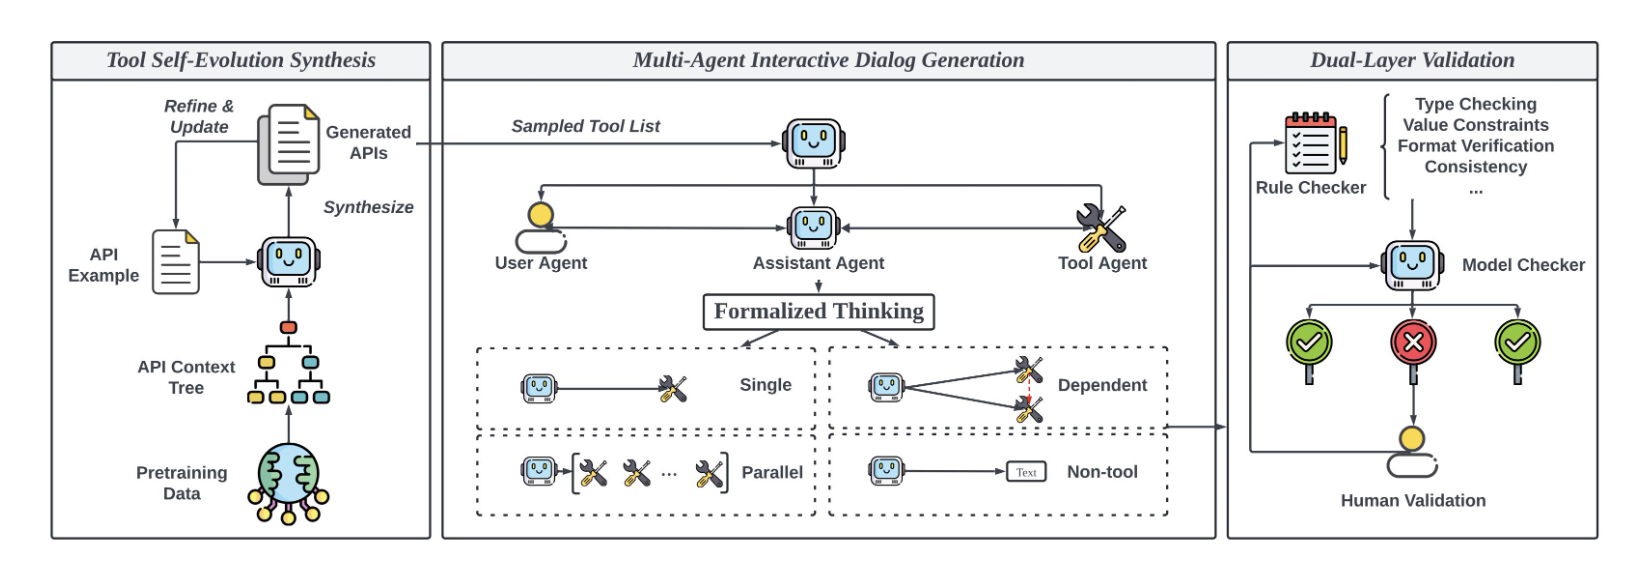
\includegraphics[height=2cm]{../assets/1.png}
%   \hspace{1cm}
%   \includegraphics[height=2cm]{sjtu-vi-badge-red.pdf}
%   \bicaption{中文题图}{English caption}
%   \label{fig:SRR}
% \end{figure}

如果多个图形相互独立,并不共用一个图形计数器,那么用 \texttt{minipage} 或者
% \texttt{parbox} 就可以,如图~\ref{fig:parallel1} 与图~\ref{fig:parallel2}。

% \begin{figure}[!htp]
%   \centering
%   \begin{minipage}{0.48\textwidth}
%     \centering
%     \includegraphics[height=1.7cm]{sjtu-vi-name-red.pdf}
%     \caption{并排第一个图}
%     \label{fig:parallel1}
%   \end{minipage}\hfill
%   \begin{minipage}{0.48\textwidth}
%     \centering
%     \includegraphics[height=1.7cm]{sjtu-vi-name-red.pdf}
%     \caption{并排第二个图}
%     \label{fig:parallel2}
%   \end{minipage}
% \end{figure}

% 如果要为共用一个计数器的多个子图添加子图题,建议使用较新的 \pkg{subcaption} 宏
% 包,不建议使用 \pkg{subfigure} 或 \pkg{subfig} 等宏包。

% 推荐使用 \pkg{subcaption} 宏包的 \cs{subcaptionbox} 并排子图,子图题置于子图之
% 下,子图号用 a)、b) 等表示。也可以使用 \pkg{subcaption} 宏包的 \cs{subcaption}
% (放在 minipage中,用法同 \cs{caption})。

% \pkg{subcaption} 宏包也提供了 \pkg{subfigure} 和 \pkg{subtable} 环境,如
% 图~\ref{fig:subfigure}。

% \begin{figure}[!htp]
%   \centering
%   \begin{subfigure}{0.3\textwidth}
%     \centering
%     \includegraphics[height=2cm]{sjtu-vi-badge-red.pdf}
%     \caption{校徽}
%   \end{subfigure}
%   \hspace{1cm}
%   \begin{subfigure}{0.4\textwidth}
%     \centering
%     \includegraphics[height=1.7cm]{sjtu-vi-name-red.pdf}
%     \caption{校名。注意这个图略矮些,subfigure 中同一行的子图在顶端对齐。}
%   \end{subfigure}
%   \caption{包含子图题的范例(使用 subfigure)}
%   \label{fig:subfigure}
% \end{figure}

% 搭配 \pkg{bicaption} 宏包时,可以启用 \cs{subcaptionbox} 和 \cs{subcaption} 的双
% 语变种 \cs{bisubcaptionbox} 和 \cs{bisubcaption},如图~\ref{fig:bisubcaptionbox}
% 所示。

% \begin{figure}[!hbtp]
%   \centering
%   \bisubcaptionbox{$R_3 = 1.5\text{mm}$ 时轴承的压力分布云图}%
%                   {Pressure contour of bearing when $R_3 = 1.5\text{mm}$}%
%                   [6.4cm]{\includegraphics[height=3cm]{example-image-a.pdf}}
%   \hspace{1cm}
%   \bisubcaptionbox{$R_3 = 2.5\text{mm}$ 时轴承的压力分布云图}%
%                   {Pressure contour of bearing when $R_3 = 2.5\text{mm}$}%
%                   [6.4cm]{\includegraphics[height=3cm]{example-image-b.pdf}}
%   \bicaption{包含子图题的范例(使用 subcaptionbox)}
%             {Example with subcaptionbox}
%   \label{fig:bisubcaptionbox}
% \end{figure}


% \section{表格}

% \subsection{基本表格}

% 编排表格应简单明了,表达一致,明晰易懂,表文呼应、内容一致。表题置于表上,研究生
% 学位论文可以用中、英文两种文字居中排写,中文在上,也可以只用中文。

% 表格的编排建议采用国际通行的三线表\footnote{三线表,以其形式简洁、功能分明、阅读
% 方便而在科技论文中被推荐使用。三线表通常只有 3 条线,即顶线、底线和栏目线,没有
% 竖线。}。三线表可以使用 \pkg{booktabs} 提供的 \cs{toprule}、\cs{midrule} 和
% \cs{bottomrule}。它们与 \pkg{longtable} 能很好的配合使用。


% \begin{table}[!hpt]
%   \caption[一个颇为标准的三线表]{一个颇为标准的三线表\footnotemark}
%   \label{tab:firstone}
%   \centering
%   \begin{tabular}{@{}llr@{}} \toprule
%     \multicolumn{2}{c}{Item} \\ \cmidrule(r){1-2}
%     Animal & Description & Price (\$)\\ \midrule
%     Gnat  & per gram  & 13.65 \\
%           & each      & 0.01 \\
%     Gnu   & stuffed   & 92.50 \\
%     Emu   & stuffed   & 33.33 \\
%     Armadillo & frozen & 8.99 \\ \bottomrule
%   \end{tabular}
% \end{table}
% \footnotetext{这个例子来自
%   \href{https://mirrors.sjtug.sjtu.edu.cn/ctan/macros/latex/contrib/booktabs/booktabs.pdf}%
%   {《Publication quality tables in LaTeX》}(\pkg{booktabs} 宏包的文档)。这也是
%   一个在表格中使用脚注的例子,请留意与 \pkg{threeparttable} 实现的效果有何不
%   同。}

% \subsection{复杂表格}

% 我们经常会在表格下方标注数据来源,或者对表格里面的条目进行解释。可以用
% \pkg{threeparttable} 实现带有脚注的表格,如表~\ref{tab:footnote}。

% \begin{table}[!htpb]
%   \bicaption{一个带有脚注的表格的例子}{A Table with footnotes}
%   \label{tab:footnote}
%   \centering
%   \begin{threeparttable}[b]
%      \begin{tabular}{ccd{4}cccc}
%       \toprule
%       \multirow{2}*{total} & \multicolumn{2}{c}{20\tnote{a}} & \multicolumn{2}{c}{40} & \multicolumn{2}{c}{60} \\
%       \cmidrule(lr){2-3}\cmidrule(lr){4-5}\cmidrule(lr){6-7}
%       & www & \multicolumn{1}{c}{k} & www & k & www & k \\ % 使用说明符 d 的列会自动进入数学模式,使用 \multicolumn 对文字表头做特殊处理
%       \midrule
%       & $\underset{(2.12)}{4.22}$ & 120.0140\tnote{b} & 333.15 & 0.0411 & 444.99 & 0.1387 \\
%       & 168.6123 & 10.86 & 255.37 & 0.0353 & 376.14 & 0.1058 \\
%       & 6.761    & 0.007 & 235.37 & 0.0267 & 348.66 & 0.1010 \\
%       \bottomrule
%     \end{tabular}
%     \begin{tablenotes}
%     \item [a] the first note.
%     \item [b] the second note.
%     \end{tablenotes}
%   \end{threeparttable}
% \end{table}


% \section{算法环境}

% 算法环境可以使用 \pkg{algorithms} 宏包或者较新的 \pkg{algorithm2e} 实现。
% 算法~\ref{algo:algorithm} 是一个使用 \pkg{algorithm2e} 的例子。关于排版算法环境
% 的具体方法,请阅读相关宏包的官方文档。

% \begin{algorithm}[htb]
%   \caption{算法示例}
%   \label{algo:algorithm}
%   \small
%   \SetAlgoLined
%   \KwData{this text}
%   \KwResult{how to write algorithm with \LaTeXe }

%   initialization\;
%   \While{not at end of this document}{
%     read current\;
%     \eIf{understand}{
%       go to next section\;
%       current section becomes this one\;
%     }{
%       go back to the beginning of current section\;
%     }
%   }
% \end{algorithm}
